%\renewcommand{\theequation}{\theenumi}
%\begin{enumerate}[label=\arabic*.,ref=\thesubsection.\theenumi]
%\numberwithin{equation}{enumi}
\item Find the equation of a circle with centre \myvec{-3\\2} and radius 4.
\\
\solution 
From the given information, the desired equation is
\begin{align}
\norm{\vec{x}-\myvec{-3\\2}}^2 = 4^2
\\
\implies \vec{x}^T\vec{x}+\myvec{6&-4}\vec{x} -3 &=0
\end{align}
The python code for Fig. \ref{fig:4.1.1_circle} is
\begin{lstlisting}
solutions/1/codes/circle/circle1.py
\end{lstlisting}
\begin{figure}[!ht]
\centering
\includegraphics[width=\columnwidth]{./solutions/1/figs/circle/circle1.eps}
\caption{Circle using python}
\label{fig:4.1.1_circle}
\end{figure}



\item Find the centre and radius of the circle
\begin{align}
\vec{x}^T\vec{x}+\myvec{8\\10}\vec{x} -8= 0
\end{align}
%
\\
\solution 
Let the balanced version of (\ref{eq:solutions/chem/6ato balance}) be
\begin{align}
    \label{eq:solutions/chem/6abalanced}x_{1}HNO_{3}+ x_{2}Ca(OH)_{2}\to x_{3}Ca(NO_{3})_{2}+ x_{4}H_{2}O
\end{align}

which results in the following equations:
\begin{align}
    (x_{1}+ 2x_{2}-2x_{4}) H= 0\\
    (x_{1}-2x_{3}) N= 0\\
    (3x_{1}+ 2x_{2}-6x_{3}- x_{4}) O=0\\
    (x_{2}-x_{3}) Ca= 0
\end{align}

which can be expressed as
\begin{align}
    x_{1}+ 2x_{2}+ 0.x_{3} -2x_{4} = 0\\
    x_{1}+ 0.x_{2} -2x_{3} +0.x_{4}= 0\\
    3x_{1}+ 2x_{2}-6x_{3}- x_{4} =0\\
    0.x_{1} +x_{2}-x_{3} +0.x_{4}= 0
\end{align}

resulting in the matrix equation
\begin{align}
    \label{eq:solutions/chem/6a matrix}
    \myvec{1 & 2 & 0 & -2\\
           1 & 0 & -2 & 0\\
           3 & 2 & -6 & -1\\
           0 & 1 & -1 & 0}\vec{x}
           =\vec{0}
\end{align}

where,
\begin{align}
   \vec{x}= \myvec{x_{1}\\x_{2}\\x_{3}\\x_{4}}
\end{align}

(\ref{eq:solutions/chem/6a matrix}) can be reduced as follows:
\begin{align}
    \myvec{1 & 2 & 0 & -2\\
           1 & 0 & -2 & 0\\
           3 & 2 & -6 & -1\\
           0 & 1 & -1 & 0}
    \xleftrightarrow[R_{3}\leftarrow \frac{R_3}{3}-R_{1}]{R_{2}\leftarrow R_2- R_1}
    \myvec{1 & 2 & 0 & -2\\
           0 & -2 & -2 & 2\\
           0 & -\frac{4}{3} & -2 & \frac{5}{3}\\
           0 & 1 & -1 & 0}\\
    \xleftrightarrow{R_2 \leftarrow -\frac{R_2}{2}}
    \myvec{1 & 2 & 0 & -2\\
          0 & 1 & 1 & -1\\
          0 & -\frac{4}{3} & -2 & \frac{5}{3}\\
          0 & 1 & -1 & 0}\\
    \xleftrightarrow[R_4 \leftarrow R_4- R_2]{R_3 \leftarrow R_3 + \frac{4}{3}R_2}
    \myvec{1 & 2 & 0 & -2\\
           0 & 1 & 1 & -1\\
           0 & 0 & -\frac{2}{3} & \frac{1}{3}\\
           0 & 0 & -2 & 1}\\
    \xleftrightarrow[R_3 \leftarrow -\frac{3}{2}R_3]{R_1 \leftarrow R_1- 2R_2}
    \myvec{1 & 0 & -2 & 0\\
           0 & 1 & 1 & -1\\
           0 & 0 & 1 & -\frac{1}{2}\\
           0 & 0 & -2 & 1}\\
    \xleftrightarrow{R_4\leftarrow R_4 + 2R_3}
    \myvec{1 & 0 & -2 & 0\\
           0 & 1 & 1 & -1\\
           0 & 0 & 1 & -\frac{1}{2}\\
           0 & 0 & 0 & 0}\\
    \xleftrightarrow[R_2\leftarrow R_2-R_3]{R_1\leftarrow R_1 + 2R_3}
    \myvec{1 & 0 & 0 & -1\\
           0 & 1 & 0 & -\frac{1}{2}\\
           0 & 0 & 1 & -\frac{1}{2}\\
           0 & 0 & 0 & 0}
\end{align}

Thus,
\begin{align}
    x_1=x_4, x_2= \frac{1}{2}x_4, x_3=\frac{1}{2}x_4\\
    \implies \quad\vec{x}= x_4\myvec{1\\ \frac{1}{2}\\ \frac{1}{2}\\1} =\myvec{2\\1\\1\\2}
\end{align} 
by substituting $x_4= 2$.

\hfill\break
%\vspace{5mm} 
Hence, (\ref{eq:solutions/chem/6abalanced}) finally becomes
\begin{align}
    2HNO_{3}+ Ca(OH)_{2}\to Ca(NO_{3})_{2}+ 2H_{2}O
\end{align}

\item Find the equation of the circle which passes through the points \myvec{2\\-2} and \myvec{3\\4} and whose centre lies on the line 
\begin{align}
\label{eq:4.1.3_line}
\myvec{1 & 1} \vec{x} = 2.
\end{align}
\\
\solution 
Let the balanced version of (\ref{eq:solutions/chem/6ato balance}) be
\begin{align}
    \label{eq:solutions/chem/6abalanced}x_{1}HNO_{3}+ x_{2}Ca(OH)_{2}\to x_{3}Ca(NO_{3})_{2}+ x_{4}H_{2}O
\end{align}

which results in the following equations:
\begin{align}
    (x_{1}+ 2x_{2}-2x_{4}) H= 0\\
    (x_{1}-2x_{3}) N= 0\\
    (3x_{1}+ 2x_{2}-6x_{3}- x_{4}) O=0\\
    (x_{2}-x_{3}) Ca= 0
\end{align}

which can be expressed as
\begin{align}
    x_{1}+ 2x_{2}+ 0.x_{3} -2x_{4} = 0\\
    x_{1}+ 0.x_{2} -2x_{3} +0.x_{4}= 0\\
    3x_{1}+ 2x_{2}-6x_{3}- x_{4} =0\\
    0.x_{1} +x_{2}-x_{3} +0.x_{4}= 0
\end{align}

resulting in the matrix equation
\begin{align}
    \label{eq:solutions/chem/6a matrix}
    \myvec{1 & 2 & 0 & -2\\
           1 & 0 & -2 & 0\\
           3 & 2 & -6 & -1\\
           0 & 1 & -1 & 0}\vec{x}
           =\vec{0}
\end{align}

where,
\begin{align}
   \vec{x}= \myvec{x_{1}\\x_{2}\\x_{3}\\x_{4}}
\end{align}

(\ref{eq:solutions/chem/6a matrix}) can be reduced as follows:
\begin{align}
    \myvec{1 & 2 & 0 & -2\\
           1 & 0 & -2 & 0\\
           3 & 2 & -6 & -1\\
           0 & 1 & -1 & 0}
    \xleftrightarrow[R_{3}\leftarrow \frac{R_3}{3}-R_{1}]{R_{2}\leftarrow R_2- R_1}
    \myvec{1 & 2 & 0 & -2\\
           0 & -2 & -2 & 2\\
           0 & -\frac{4}{3} & -2 & \frac{5}{3}\\
           0 & 1 & -1 & 0}\\
    \xleftrightarrow{R_2 \leftarrow -\frac{R_2}{2}}
    \myvec{1 & 2 & 0 & -2\\
          0 & 1 & 1 & -1\\
          0 & -\frac{4}{3} & -2 & \frac{5}{3}\\
          0 & 1 & -1 & 0}\\
    \xleftrightarrow[R_4 \leftarrow R_4- R_2]{R_3 \leftarrow R_3 + \frac{4}{3}R_2}
    \myvec{1 & 2 & 0 & -2\\
           0 & 1 & 1 & -1\\
           0 & 0 & -\frac{2}{3} & \frac{1}{3}\\
           0 & 0 & -2 & 1}\\
    \xleftrightarrow[R_3 \leftarrow -\frac{3}{2}R_3]{R_1 \leftarrow R_1- 2R_2}
    \myvec{1 & 0 & -2 & 0\\
           0 & 1 & 1 & -1\\
           0 & 0 & 1 & -\frac{1}{2}\\
           0 & 0 & -2 & 1}\\
    \xleftrightarrow{R_4\leftarrow R_4 + 2R_3}
    \myvec{1 & 0 & -2 & 0\\
           0 & 1 & 1 & -1\\
           0 & 0 & 1 & -\frac{1}{2}\\
           0 & 0 & 0 & 0}\\
    \xleftrightarrow[R_2\leftarrow R_2-R_3]{R_1\leftarrow R_1 + 2R_3}
    \myvec{1 & 0 & 0 & -1\\
           0 & 1 & 0 & -\frac{1}{2}\\
           0 & 0 & 1 & -\frac{1}{2}\\
           0 & 0 & 0 & 0}
\end{align}

Thus,
\begin{align}
    x_1=x_4, x_2= \frac{1}{2}x_4, x_3=\frac{1}{2}x_4\\
    \implies \quad\vec{x}= x_4\myvec{1\\ \frac{1}{2}\\ \frac{1}{2}\\1} =\myvec{2\\1\\1\\2}
\end{align} 
by substituting $x_4= 2$.

\hfill\break
%\vspace{5mm} 
Hence, (\ref{eq:solutions/chem/6abalanced}) finally becomes
\begin{align}
    2HNO_{3}+ Ca(OH)_{2}\to Ca(NO_{3})_{2}+ 2H_{2}O
\end{align}

\item Find the area enclosed by the circle $\norm{\vec{x}} = a$
%
\\
\solution The area is $2\pi a^2$.
%
\item Find the area of the region in the first quadrant enclosed by the x-axis, the line $\myvec{1 & -1}\vec{x} = 0$, and the circle $\norm{\vec{x}} = 1$.
%
\\
\solution 
Let the balanced version of (\ref{eq:solutions/chem/6ato balance}) be
\begin{align}
    \label{eq:solutions/chem/6abalanced}x_{1}HNO_{3}+ x_{2}Ca(OH)_{2}\to x_{3}Ca(NO_{3})_{2}+ x_{4}H_{2}O
\end{align}

which results in the following equations:
\begin{align}
    (x_{1}+ 2x_{2}-2x_{4}) H= 0\\
    (x_{1}-2x_{3}) N= 0\\
    (3x_{1}+ 2x_{2}-6x_{3}- x_{4}) O=0\\
    (x_{2}-x_{3}) Ca= 0
\end{align}

which can be expressed as
\begin{align}
    x_{1}+ 2x_{2}+ 0.x_{3} -2x_{4} = 0\\
    x_{1}+ 0.x_{2} -2x_{3} +0.x_{4}= 0\\
    3x_{1}+ 2x_{2}-6x_{3}- x_{4} =0\\
    0.x_{1} +x_{2}-x_{3} +0.x_{4}= 0
\end{align}

resulting in the matrix equation
\begin{align}
    \label{eq:solutions/chem/6a matrix}
    \myvec{1 & 2 & 0 & -2\\
           1 & 0 & -2 & 0\\
           3 & 2 & -6 & -1\\
           0 & 1 & -1 & 0}\vec{x}
           =\vec{0}
\end{align}

where,
\begin{align}
   \vec{x}= \myvec{x_{1}\\x_{2}\\x_{3}\\x_{4}}
\end{align}

(\ref{eq:solutions/chem/6a matrix}) can be reduced as follows:
\begin{align}
    \myvec{1 & 2 & 0 & -2\\
           1 & 0 & -2 & 0\\
           3 & 2 & -6 & -1\\
           0 & 1 & -1 & 0}
    \xleftrightarrow[R_{3}\leftarrow \frac{R_3}{3}-R_{1}]{R_{2}\leftarrow R_2- R_1}
    \myvec{1 & 2 & 0 & -2\\
           0 & -2 & -2 & 2\\
           0 & -\frac{4}{3} & -2 & \frac{5}{3}\\
           0 & 1 & -1 & 0}\\
    \xleftrightarrow{R_2 \leftarrow -\frac{R_2}{2}}
    \myvec{1 & 2 & 0 & -2\\
          0 & 1 & 1 & -1\\
          0 & -\frac{4}{3} & -2 & \frac{5}{3}\\
          0 & 1 & -1 & 0}\\
    \xleftrightarrow[R_4 \leftarrow R_4- R_2]{R_3 \leftarrow R_3 + \frac{4}{3}R_2}
    \myvec{1 & 2 & 0 & -2\\
           0 & 1 & 1 & -1\\
           0 & 0 & -\frac{2}{3} & \frac{1}{3}\\
           0 & 0 & -2 & 1}\\
    \xleftrightarrow[R_3 \leftarrow -\frac{3}{2}R_3]{R_1 \leftarrow R_1- 2R_2}
    \myvec{1 & 0 & -2 & 0\\
           0 & 1 & 1 & -1\\
           0 & 0 & 1 & -\frac{1}{2}\\
           0 & 0 & -2 & 1}\\
    \xleftrightarrow{R_4\leftarrow R_4 + 2R_3}
    \myvec{1 & 0 & -2 & 0\\
           0 & 1 & 1 & -1\\
           0 & 0 & 1 & -\frac{1}{2}\\
           0 & 0 & 0 & 0}\\
    \xleftrightarrow[R_2\leftarrow R_2-R_3]{R_1\leftarrow R_1 + 2R_3}
    \myvec{1 & 0 & 0 & -1\\
           0 & 1 & 0 & -\frac{1}{2}\\
           0 & 0 & 1 & -\frac{1}{2}\\
           0 & 0 & 0 & 0}
\end{align}

Thus,
\begin{align}
    x_1=x_4, x_2= \frac{1}{2}x_4, x_3=\frac{1}{2}x_4\\
    \implies \quad\vec{x}= x_4\myvec{1\\ \frac{1}{2}\\ \frac{1}{2}\\1} =\myvec{2\\1\\1\\2}
\end{align} 
by substituting $x_4= 2$.

\hfill\break
%\vspace{5mm} 
Hence, (\ref{eq:solutions/chem/6abalanced}) finally becomes
\begin{align}
    2HNO_{3}+ Ca(OH)_{2}\to Ca(NO_{3})_{2}+ 2H_{2}O
\end{align}

%
\item Find the area of the region enclosed between the two circles: $\vec{x}^T\vec{x} = 4$ and $\norm{\vec{x}-\myvec{2\\0}} = 2$.
%
\item Find the coordinates of a point $\vec{A}$, where $AB$ is the diameter of a circle whose centre is \myvec{2,-3} and $\vec{B} = \myvec{1\\4}$.
\\
\solution 
Let the balanced version of (\ref{eq:solutions/chem/6ato balance}) be
\begin{align}
    \label{eq:solutions/chem/6abalanced}x_{1}HNO_{3}+ x_{2}Ca(OH)_{2}\to x_{3}Ca(NO_{3})_{2}+ x_{4}H_{2}O
\end{align}

which results in the following equations:
\begin{align}
    (x_{1}+ 2x_{2}-2x_{4}) H= 0\\
    (x_{1}-2x_{3}) N= 0\\
    (3x_{1}+ 2x_{2}-6x_{3}- x_{4}) O=0\\
    (x_{2}-x_{3}) Ca= 0
\end{align}

which can be expressed as
\begin{align}
    x_{1}+ 2x_{2}+ 0.x_{3} -2x_{4} = 0\\
    x_{1}+ 0.x_{2} -2x_{3} +0.x_{4}= 0\\
    3x_{1}+ 2x_{2}-6x_{3}- x_{4} =0\\
    0.x_{1} +x_{2}-x_{3} +0.x_{4}= 0
\end{align}

resulting in the matrix equation
\begin{align}
    \label{eq:solutions/chem/6a matrix}
    \myvec{1 & 2 & 0 & -2\\
           1 & 0 & -2 & 0\\
           3 & 2 & -6 & -1\\
           0 & 1 & -1 & 0}\vec{x}
           =\vec{0}
\end{align}

where,
\begin{align}
   \vec{x}= \myvec{x_{1}\\x_{2}\\x_{3}\\x_{4}}
\end{align}

(\ref{eq:solutions/chem/6a matrix}) can be reduced as follows:
\begin{align}
    \myvec{1 & 2 & 0 & -2\\
           1 & 0 & -2 & 0\\
           3 & 2 & -6 & -1\\
           0 & 1 & -1 & 0}
    \xleftrightarrow[R_{3}\leftarrow \frac{R_3}{3}-R_{1}]{R_{2}\leftarrow R_2- R_1}
    \myvec{1 & 2 & 0 & -2\\
           0 & -2 & -2 & 2\\
           0 & -\frac{4}{3} & -2 & \frac{5}{3}\\
           0 & 1 & -1 & 0}\\
    \xleftrightarrow{R_2 \leftarrow -\frac{R_2}{2}}
    \myvec{1 & 2 & 0 & -2\\
          0 & 1 & 1 & -1\\
          0 & -\frac{4}{3} & -2 & \frac{5}{3}\\
          0 & 1 & -1 & 0}\\
    \xleftrightarrow[R_4 \leftarrow R_4- R_2]{R_3 \leftarrow R_3 + \frac{4}{3}R_2}
    \myvec{1 & 2 & 0 & -2\\
           0 & 1 & 1 & -1\\
           0 & 0 & -\frac{2}{3} & \frac{1}{3}\\
           0 & 0 & -2 & 1}\\
    \xleftrightarrow[R_3 \leftarrow -\frac{3}{2}R_3]{R_1 \leftarrow R_1- 2R_2}
    \myvec{1 & 0 & -2 & 0\\
           0 & 1 & 1 & -1\\
           0 & 0 & 1 & -\frac{1}{2}\\
           0 & 0 & -2 & 1}\\
    \xleftrightarrow{R_4\leftarrow R_4 + 2R_3}
    \myvec{1 & 0 & -2 & 0\\
           0 & 1 & 1 & -1\\
           0 & 0 & 1 & -\frac{1}{2}\\
           0 & 0 & 0 & 0}\\
    \xleftrightarrow[R_2\leftarrow R_2-R_3]{R_1\leftarrow R_1 + 2R_3}
    \myvec{1 & 0 & 0 & -1\\
           0 & 1 & 0 & -\frac{1}{2}\\
           0 & 0 & 1 & -\frac{1}{2}\\
           0 & 0 & 0 & 0}
\end{align}

Thus,
\begin{align}
    x_1=x_4, x_2= \frac{1}{2}x_4, x_3=\frac{1}{2}x_4\\
    \implies \quad\vec{x}= x_4\myvec{1\\ \frac{1}{2}\\ \frac{1}{2}\\1} =\myvec{2\\1\\1\\2}
\end{align} 
by substituting $x_4= 2$.

\hfill\break
%\vspace{5mm} 
Hence, (\ref{eq:solutions/chem/6abalanced}) finally becomes
\begin{align}
    2HNO_{3}+ Ca(OH)_{2}\to Ca(NO_{3})_{2}+ 2H_{2}O
\end{align}

\item Find the centre $O$ of a circle passing through the points \myvec{6\\-6}, \myvec{3\\-7} and  \myvec{3\\3}.
\solution 
Let the balanced version of (\ref{eq:solutions/chem/6ato balance}) be
\begin{align}
    \label{eq:solutions/chem/6abalanced}x_{1}HNO_{3}+ x_{2}Ca(OH)_{2}\to x_{3}Ca(NO_{3})_{2}+ x_{4}H_{2}O
\end{align}

which results in the following equations:
\begin{align}
    (x_{1}+ 2x_{2}-2x_{4}) H= 0\\
    (x_{1}-2x_{3}) N= 0\\
    (3x_{1}+ 2x_{2}-6x_{3}- x_{4}) O=0\\
    (x_{2}-x_{3}) Ca= 0
\end{align}

which can be expressed as
\begin{align}
    x_{1}+ 2x_{2}+ 0.x_{3} -2x_{4} = 0\\
    x_{1}+ 0.x_{2} -2x_{3} +0.x_{4}= 0\\
    3x_{1}+ 2x_{2}-6x_{3}- x_{4} =0\\
    0.x_{1} +x_{2}-x_{3} +0.x_{4}= 0
\end{align}

resulting in the matrix equation
\begin{align}
    \label{eq:solutions/chem/6a matrix}
    \myvec{1 & 2 & 0 & -2\\
           1 & 0 & -2 & 0\\
           3 & 2 & -6 & -1\\
           0 & 1 & -1 & 0}\vec{x}
           =\vec{0}
\end{align}

where,
\begin{align}
   \vec{x}= \myvec{x_{1}\\x_{2}\\x_{3}\\x_{4}}
\end{align}

(\ref{eq:solutions/chem/6a matrix}) can be reduced as follows:
\begin{align}
    \myvec{1 & 2 & 0 & -2\\
           1 & 0 & -2 & 0\\
           3 & 2 & -6 & -1\\
           0 & 1 & -1 & 0}
    \xleftrightarrow[R_{3}\leftarrow \frac{R_3}{3}-R_{1}]{R_{2}\leftarrow R_2- R_1}
    \myvec{1 & 2 & 0 & -2\\
           0 & -2 & -2 & 2\\
           0 & -\frac{4}{3} & -2 & \frac{5}{3}\\
           0 & 1 & -1 & 0}\\
    \xleftrightarrow{R_2 \leftarrow -\frac{R_2}{2}}
    \myvec{1 & 2 & 0 & -2\\
          0 & 1 & 1 & -1\\
          0 & -\frac{4}{3} & -2 & \frac{5}{3}\\
          0 & 1 & -1 & 0}\\
    \xleftrightarrow[R_4 \leftarrow R_4- R_2]{R_3 \leftarrow R_3 + \frac{4}{3}R_2}
    \myvec{1 & 2 & 0 & -2\\
           0 & 1 & 1 & -1\\
           0 & 0 & -\frac{2}{3} & \frac{1}{3}\\
           0 & 0 & -2 & 1}\\
    \xleftrightarrow[R_3 \leftarrow -\frac{3}{2}R_3]{R_1 \leftarrow R_1- 2R_2}
    \myvec{1 & 0 & -2 & 0\\
           0 & 1 & 1 & -1\\
           0 & 0 & 1 & -\frac{1}{2}\\
           0 & 0 & -2 & 1}\\
    \xleftrightarrow{R_4\leftarrow R_4 + 2R_3}
    \myvec{1 & 0 & -2 & 0\\
           0 & 1 & 1 & -1\\
           0 & 0 & 1 & -\frac{1}{2}\\
           0 & 0 & 0 & 0}\\
    \xleftrightarrow[R_2\leftarrow R_2-R_3]{R_1\leftarrow R_1 + 2R_3}
    \myvec{1 & 0 & 0 & -1\\
           0 & 1 & 0 & -\frac{1}{2}\\
           0 & 0 & 1 & -\frac{1}{2}\\
           0 & 0 & 0 & 0}
\end{align}

Thus,
\begin{align}
    x_1=x_4, x_2= \frac{1}{2}x_4, x_3=\frac{1}{2}x_4\\
    \implies \quad\vec{x}= x_4\myvec{1\\ \frac{1}{2}\\ \frac{1}{2}\\1} =\myvec{2\\1\\1\\2}
\end{align} 
by substituting $x_4= 2$.

\hfill\break
%\vspace{5mm} 
Hence, (\ref{eq:solutions/chem/6abalanced}) finally becomes
\begin{align}
    2HNO_{3}+ Ca(OH)_{2}\to Ca(NO_{3})_{2}+ 2H_{2}O
\end{align}

\item Sketch the circles with 
\begin{enumerate}
\item centre \myvec{0\\2} and radius 2
\item centre \myvec{-2\\32} and radius 4
\item centre $\myvec{\frac{1}{2}\\ \frac{1}{4}}$ and radius $\frac{1}{12}$.
\item centre \myvec{1\\1} and radius $\sqrt{2}$.
\item centre \myvec{-a\\-b} and radius $\sqrt{a^2-b^2}$.
\end{enumerate}
\solution 
Let the balanced version of (\ref{eq:solutions/chem/6ato balance}) be
\begin{align}
    \label{eq:solutions/chem/6abalanced}x_{1}HNO_{3}+ x_{2}Ca(OH)_{2}\to x_{3}Ca(NO_{3})_{2}+ x_{4}H_{2}O
\end{align}

which results in the following equations:
\begin{align}
    (x_{1}+ 2x_{2}-2x_{4}) H= 0\\
    (x_{1}-2x_{3}) N= 0\\
    (3x_{1}+ 2x_{2}-6x_{3}- x_{4}) O=0\\
    (x_{2}-x_{3}) Ca= 0
\end{align}

which can be expressed as
\begin{align}
    x_{1}+ 2x_{2}+ 0.x_{3} -2x_{4} = 0\\
    x_{1}+ 0.x_{2} -2x_{3} +0.x_{4}= 0\\
    3x_{1}+ 2x_{2}-6x_{3}- x_{4} =0\\
    0.x_{1} +x_{2}-x_{3} +0.x_{4}= 0
\end{align}

resulting in the matrix equation
\begin{align}
    \label{eq:solutions/chem/6a matrix}
    \myvec{1 & 2 & 0 & -2\\
           1 & 0 & -2 & 0\\
           3 & 2 & -6 & -1\\
           0 & 1 & -1 & 0}\vec{x}
           =\vec{0}
\end{align}

where,
\begin{align}
   \vec{x}= \myvec{x_{1}\\x_{2}\\x_{3}\\x_{4}}
\end{align}

(\ref{eq:solutions/chem/6a matrix}) can be reduced as follows:
\begin{align}
    \myvec{1 & 2 & 0 & -2\\
           1 & 0 & -2 & 0\\
           3 & 2 & -6 & -1\\
           0 & 1 & -1 & 0}
    \xleftrightarrow[R_{3}\leftarrow \frac{R_3}{3}-R_{1}]{R_{2}\leftarrow R_2- R_1}
    \myvec{1 & 2 & 0 & -2\\
           0 & -2 & -2 & 2\\
           0 & -\frac{4}{3} & -2 & \frac{5}{3}\\
           0 & 1 & -1 & 0}\\
    \xleftrightarrow{R_2 \leftarrow -\frac{R_2}{2}}
    \myvec{1 & 2 & 0 & -2\\
          0 & 1 & 1 & -1\\
          0 & -\frac{4}{3} & -2 & \frac{5}{3}\\
          0 & 1 & -1 & 0}\\
    \xleftrightarrow[R_4 \leftarrow R_4- R_2]{R_3 \leftarrow R_3 + \frac{4}{3}R_2}
    \myvec{1 & 2 & 0 & -2\\
           0 & 1 & 1 & -1\\
           0 & 0 & -\frac{2}{3} & \frac{1}{3}\\
           0 & 0 & -2 & 1}\\
    \xleftrightarrow[R_3 \leftarrow -\frac{3}{2}R_3]{R_1 \leftarrow R_1- 2R_2}
    \myvec{1 & 0 & -2 & 0\\
           0 & 1 & 1 & -1\\
           0 & 0 & 1 & -\frac{1}{2}\\
           0 & 0 & -2 & 1}\\
    \xleftrightarrow{R_4\leftarrow R_4 + 2R_3}
    \myvec{1 & 0 & -2 & 0\\
           0 & 1 & 1 & -1\\
           0 & 0 & 1 & -\frac{1}{2}\\
           0 & 0 & 0 & 0}\\
    \xleftrightarrow[R_2\leftarrow R_2-R_3]{R_1\leftarrow R_1 + 2R_3}
    \myvec{1 & 0 & 0 & -1\\
           0 & 1 & 0 & -\frac{1}{2}\\
           0 & 0 & 1 & -\frac{1}{2}\\
           0 & 0 & 0 & 0}
\end{align}

Thus,
\begin{align}
    x_1=x_4, x_2= \frac{1}{2}x_4, x_3=\frac{1}{2}x_4\\
    \implies \quad\vec{x}= x_4\myvec{1\\ \frac{1}{2}\\ \frac{1}{2}\\1} =\myvec{2\\1\\1\\2}
\end{align} 
by substituting $x_4= 2$.

\hfill\break
%\vspace{5mm} 
Hence, (\ref{eq:solutions/chem/6abalanced}) finally becomes
\begin{align}
    2HNO_{3}+ Ca(OH)_{2}\to Ca(NO_{3})_{2}+ 2H_{2}O
\end{align}

\item  Does the point \myvec{–2.5\\ 3.5} lie inside, outside or on the circle $\vec{x}^T\vec{x} = 25$?
\\
\solution 
From the given information, the desired equation is
\begin{align}
\norm{\vec{x}-\myvec{-3\\2}}^2 = 4^2
\\
\implies \vec{x}^T\vec{x}+\myvec{6&-4}\vec{x} -3 &=0
\end{align}
The python code for Fig. \ref{fig:4.1.1_circle} is
\begin{lstlisting}
solutions/1/codes/circle/circle1.py
\end{lstlisting}
\begin{figure}[!ht]
\centering
\includegraphics[width=\columnwidth]{./solutions/1/figs/circle/circle1.eps}
\caption{Circle using python}
\label{fig:4.1.1_circle}
\end{figure}


\item Sketch the circles with equation
\begin{enumerate}
\item $\norm{\vec{x}-\myvec{5\\-3}}^2 = 36$
\item $\vec{x}^T\vec{x}-\myvec{4\\8}\vec{x} -45= 0$
\item $\vec{x}^T\vec{x}-\myvec{8\\-10}\vec{x} -12= 0$
\item $2\vec{x}^T\vec{x}-\myvec{1\\0}\vec{x} = 0$
\end{enumerate}
\solution 
The following python codes generate the required circle
	\begin{lstlisting}
	./solutions/5/codes/circle/q18abc.py
	./solutions/5/codes/circle/q18d.py
	\end{lstlisting}


\begin{enumerate}

\item \begin{align} 
\vec{x^Tx} - \myvec{4\\8}\vec{x} -45 = 0
\end{align}
See Fig. \ref{fig:4.2.5_qoeabc}.
\begin{align}
\vec{O} = \myvec{2\\4}, r = \sqrt{65} 
\end{align}
	\begin{figure}[!ht]
	\centering
	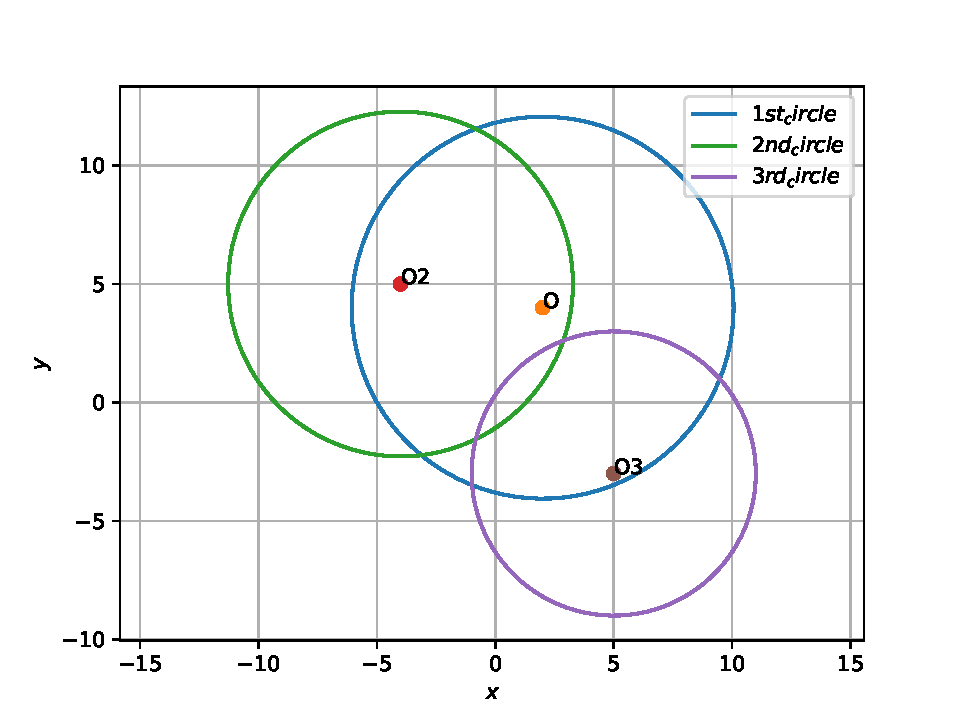
\includegraphics[width=\columnwidth]{./solutions/5/figs/circle/q18abc.eps}
	\caption{}
	\label{fig:4.2.5_qoeabc}	
	\end{figure}

\item See Fig. \ref{fig:4.2.5_qoeabc}.
\begin{align}
\vec{O} = \myvec{-4\\5}, r = \sqrt{53} 
\end{align}

\begin{align} 
\vec{x^Tx} - \myvec{8\\-10}\vec{x} - 12 = 0
\end{align}


\item See Fig. \ref{fig:4.2.5_qoeabc}.
\begin{align}
\vec{O} = \myvec{5\\-3}, r = 6
\end{align}
\begin{align} 
\norm{x - \myvec{5\\-3}} = 36
\end{align}



\begin{comment}
	\begin{figure}[!ht]
	\centering
	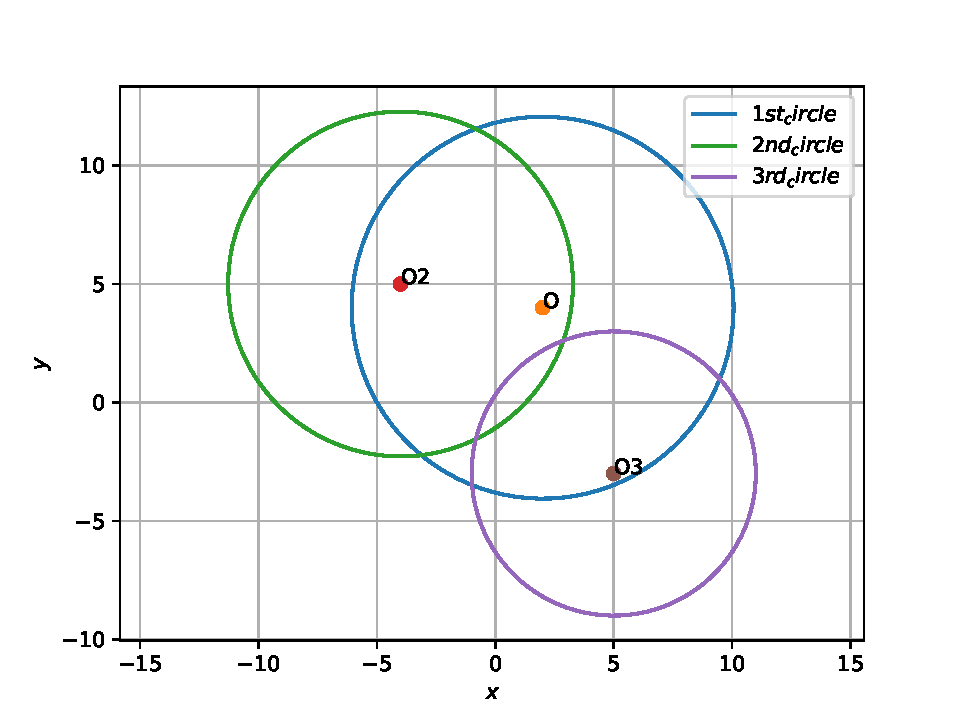
\includegraphics[width=\columnwidth]{./solutions/5/figs/circle/q18abc.eps}
	\caption{Circle of Q.4.2.5}
	\label{fig:4.2.5_qoeb}	
	\end{figure}
\end{comment}
\begin{comment}
	\begin{figure}[!ht]
	\centering
	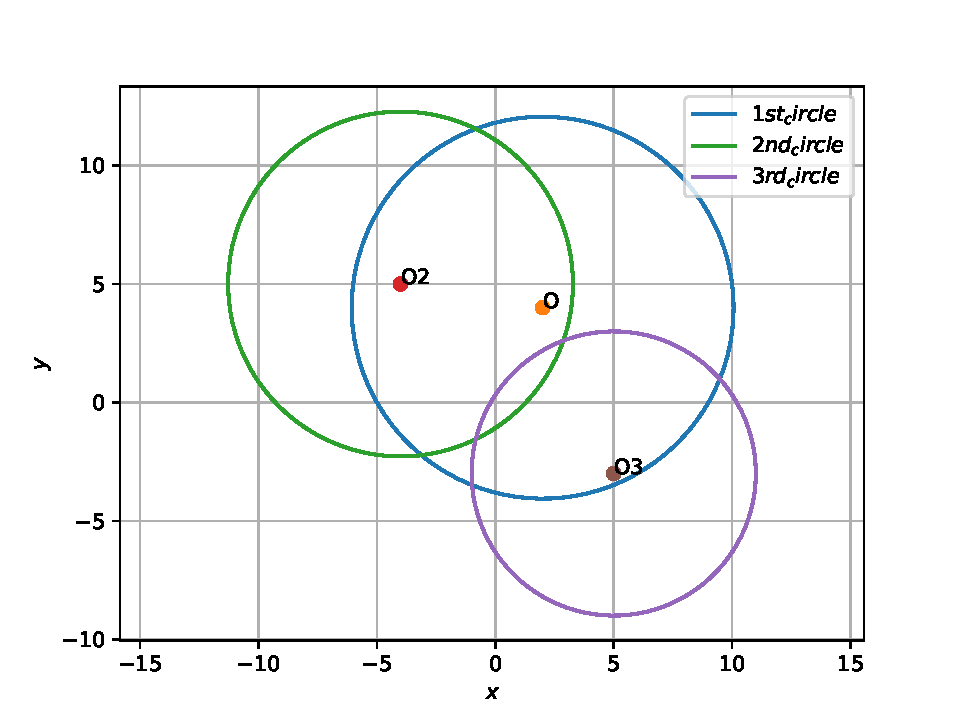
\includegraphics[width=\columnwidth]{./solutions/5/figs/circle/q18abc.eps}
	\caption{Circle of Q.4.2.5}
	\label{fig:4.2.5_qoec}	
	\end{figure}
\end{comment}
\item See Fig. \ref{fig:4.2.5_qoed}.
\begin{align}
\vec{O} = \frac{1}{4}\myvec{1\\0}, r = \frac{1}{4}
\end{align}
\begin{align} 
2\vec{x^Tx} - \myvec{1\\0}\vec{x} = 0
\end{align}
	\begin{figure}[!ht]
	\centering
	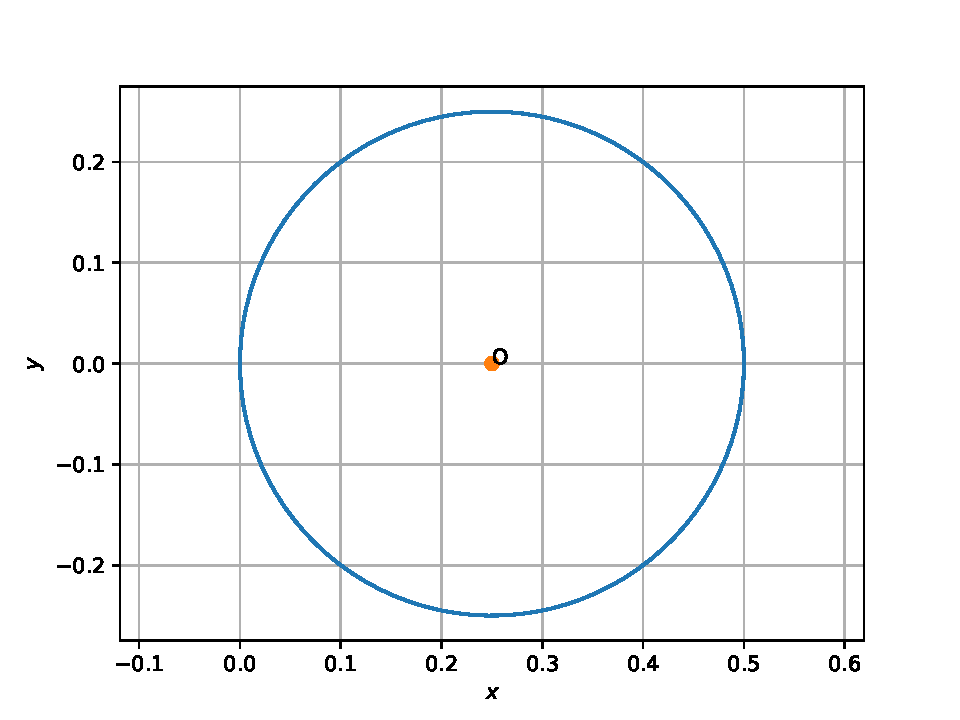
\includegraphics[width=\columnwidth]{./solutions/5/figs/circle/q18d.eps}
	\caption{}
	\label{fig:4.2.5_qoed}	
	\end{figure}



\end{enumerate}

\item Find the equation of the circle passing through the points \myvec{4\\1} and \myvec{6\\5} and whose centre is on the line $\myvec{4 & 1}\vec{x} = 16$.
\\
\solution 
Let the balanced version of (\ref{eq:solutions/chem/6ato balance}) be
\begin{align}
    \label{eq:solutions/chem/6abalanced}x_{1}HNO_{3}+ x_{2}Ca(OH)_{2}\to x_{3}Ca(NO_{3})_{2}+ x_{4}H_{2}O
\end{align}

which results in the following equations:
\begin{align}
    (x_{1}+ 2x_{2}-2x_{4}) H= 0\\
    (x_{1}-2x_{3}) N= 0\\
    (3x_{1}+ 2x_{2}-6x_{3}- x_{4}) O=0\\
    (x_{2}-x_{3}) Ca= 0
\end{align}

which can be expressed as
\begin{align}
    x_{1}+ 2x_{2}+ 0.x_{3} -2x_{4} = 0\\
    x_{1}+ 0.x_{2} -2x_{3} +0.x_{4}= 0\\
    3x_{1}+ 2x_{2}-6x_{3}- x_{4} =0\\
    0.x_{1} +x_{2}-x_{3} +0.x_{4}= 0
\end{align}

resulting in the matrix equation
\begin{align}
    \label{eq:solutions/chem/6a matrix}
    \myvec{1 & 2 & 0 & -2\\
           1 & 0 & -2 & 0\\
           3 & 2 & -6 & -1\\
           0 & 1 & -1 & 0}\vec{x}
           =\vec{0}
\end{align}

where,
\begin{align}
   \vec{x}= \myvec{x_{1}\\x_{2}\\x_{3}\\x_{4}}
\end{align}

(\ref{eq:solutions/chem/6a matrix}) can be reduced as follows:
\begin{align}
    \myvec{1 & 2 & 0 & -2\\
           1 & 0 & -2 & 0\\
           3 & 2 & -6 & -1\\
           0 & 1 & -1 & 0}
    \xleftrightarrow[R_{3}\leftarrow \frac{R_3}{3}-R_{1}]{R_{2}\leftarrow R_2- R_1}
    \myvec{1 & 2 & 0 & -2\\
           0 & -2 & -2 & 2\\
           0 & -\frac{4}{3} & -2 & \frac{5}{3}\\
           0 & 1 & -1 & 0}\\
    \xleftrightarrow{R_2 \leftarrow -\frac{R_2}{2}}
    \myvec{1 & 2 & 0 & -2\\
          0 & 1 & 1 & -1\\
          0 & -\frac{4}{3} & -2 & \frac{5}{3}\\
          0 & 1 & -1 & 0}\\
    \xleftrightarrow[R_4 \leftarrow R_4- R_2]{R_3 \leftarrow R_3 + \frac{4}{3}R_2}
    \myvec{1 & 2 & 0 & -2\\
           0 & 1 & 1 & -1\\
           0 & 0 & -\frac{2}{3} & \frac{1}{3}\\
           0 & 0 & -2 & 1}\\
    \xleftrightarrow[R_3 \leftarrow -\frac{3}{2}R_3]{R_1 \leftarrow R_1- 2R_2}
    \myvec{1 & 0 & -2 & 0\\
           0 & 1 & 1 & -1\\
           0 & 0 & 1 & -\frac{1}{2}\\
           0 & 0 & -2 & 1}\\
    \xleftrightarrow{R_4\leftarrow R_4 + 2R_3}
    \myvec{1 & 0 & -2 & 0\\
           0 & 1 & 1 & -1\\
           0 & 0 & 1 & -\frac{1}{2}\\
           0 & 0 & 0 & 0}\\
    \xleftrightarrow[R_2\leftarrow R_2-R_3]{R_1\leftarrow R_1 + 2R_3}
    \myvec{1 & 0 & 0 & -1\\
           0 & 1 & 0 & -\frac{1}{2}\\
           0 & 0 & 1 & -\frac{1}{2}\\
           0 & 0 & 0 & 0}
\end{align}

Thus,
\begin{align}
    x_1=x_4, x_2= \frac{1}{2}x_4, x_3=\frac{1}{2}x_4\\
    \implies \quad\vec{x}= x_4\myvec{1\\ \frac{1}{2}\\ \frac{1}{2}\\1} =\myvec{2\\1\\1\\2}
\end{align} 
by substituting $x_4= 2$.

\hfill\break
%\vspace{5mm} 
Hence, (\ref{eq:solutions/chem/6abalanced}) finally becomes
\begin{align}
    2HNO_{3}+ Ca(OH)_{2}\to Ca(NO_{3})_{2}+ 2H_{2}O
\end{align}

\item Find the equation of the circle passing through the points $\vec{P} =\myvec{2\\3}$ and $\vec{Q} = \myvec{–1\\1}$ and whose centre is on the line $\myvec{1 & -3}\vec{x} = 11$.
\solution 
Let the balanced version of (\ref{eq:solutions/chem/6ato balance}) be
\begin{align}
    \label{eq:solutions/chem/6abalanced}x_{1}HNO_{3}+ x_{2}Ca(OH)_{2}\to x_{3}Ca(NO_{3})_{2}+ x_{4}H_{2}O
\end{align}

which results in the following equations:
\begin{align}
    (x_{1}+ 2x_{2}-2x_{4}) H= 0\\
    (x_{1}-2x_{3}) N= 0\\
    (3x_{1}+ 2x_{2}-6x_{3}- x_{4}) O=0\\
    (x_{2}-x_{3}) Ca= 0
\end{align}

which can be expressed as
\begin{align}
    x_{1}+ 2x_{2}+ 0.x_{3} -2x_{4} = 0\\
    x_{1}+ 0.x_{2} -2x_{3} +0.x_{4}= 0\\
    3x_{1}+ 2x_{2}-6x_{3}- x_{4} =0\\
    0.x_{1} +x_{2}-x_{3} +0.x_{4}= 0
\end{align}

resulting in the matrix equation
\begin{align}
    \label{eq:solutions/chem/6a matrix}
    \myvec{1 & 2 & 0 & -2\\
           1 & 0 & -2 & 0\\
           3 & 2 & -6 & -1\\
           0 & 1 & -1 & 0}\vec{x}
           =\vec{0}
\end{align}

where,
\begin{align}
   \vec{x}= \myvec{x_{1}\\x_{2}\\x_{3}\\x_{4}}
\end{align}

(\ref{eq:solutions/chem/6a matrix}) can be reduced as follows:
\begin{align}
    \myvec{1 & 2 & 0 & -2\\
           1 & 0 & -2 & 0\\
           3 & 2 & -6 & -1\\
           0 & 1 & -1 & 0}
    \xleftrightarrow[R_{3}\leftarrow \frac{R_3}{3}-R_{1}]{R_{2}\leftarrow R_2- R_1}
    \myvec{1 & 2 & 0 & -2\\
           0 & -2 & -2 & 2\\
           0 & -\frac{4}{3} & -2 & \frac{5}{3}\\
           0 & 1 & -1 & 0}\\
    \xleftrightarrow{R_2 \leftarrow -\frac{R_2}{2}}
    \myvec{1 & 2 & 0 & -2\\
          0 & 1 & 1 & -1\\
          0 & -\frac{4}{3} & -2 & \frac{5}{3}\\
          0 & 1 & -1 & 0}\\
    \xleftrightarrow[R_4 \leftarrow R_4- R_2]{R_3 \leftarrow R_3 + \frac{4}{3}R_2}
    \myvec{1 & 2 & 0 & -2\\
           0 & 1 & 1 & -1\\
           0 & 0 & -\frac{2}{3} & \frac{1}{3}\\
           0 & 0 & -2 & 1}\\
    \xleftrightarrow[R_3 \leftarrow -\frac{3}{2}R_3]{R_1 \leftarrow R_1- 2R_2}
    \myvec{1 & 0 & -2 & 0\\
           0 & 1 & 1 & -1\\
           0 & 0 & 1 & -\frac{1}{2}\\
           0 & 0 & -2 & 1}\\
    \xleftrightarrow{R_4\leftarrow R_4 + 2R_3}
    \myvec{1 & 0 & -2 & 0\\
           0 & 1 & 1 & -1\\
           0 & 0 & 1 & -\frac{1}{2}\\
           0 & 0 & 0 & 0}\\
    \xleftrightarrow[R_2\leftarrow R_2-R_3]{R_1\leftarrow R_1 + 2R_3}
    \myvec{1 & 0 & 0 & -1\\
           0 & 1 & 0 & -\frac{1}{2}\\
           0 & 0 & 1 & -\frac{1}{2}\\
           0 & 0 & 0 & 0}
\end{align}

Thus,
\begin{align}
    x_1=x_4, x_2= \frac{1}{2}x_4, x_3=\frac{1}{2}x_4\\
    \implies \quad\vec{x}= x_4\myvec{1\\ \frac{1}{2}\\ \frac{1}{2}\\1} =\myvec{2\\1\\1\\2}
\end{align} 
by substituting $x_4= 2$.

\hfill\break
%\vspace{5mm} 
Hence, (\ref{eq:solutions/chem/6abalanced}) finally becomes
\begin{align}
    2HNO_{3}+ Ca(OH)_{2}\to Ca(NO_{3})_{2}+ 2H_{2}O
\end{align}

%\end{enumerate}
